\documentclass{beamer}
\usepackage[spanish]{babel}
\usepackage{tikz} 
\usepackage{tikz-network}
\usepackage[utf8]{inputenc}
\usepackage{hyperref}
\usepackage{algorithm,algorithmic}
\usetheme{CambridgeUS}
\usepackage{natbib}
\title{Uso de Q-learning y redes neuronales como alternativa a la solución del problema flexible scheduling}
\author{Lic. Arnoldo Del Toro Peña }
\institute{Universidad Autónoma de Nuevo León}
\begin{document}

\begin{frame}
 \titlepage
\end{frame}

\begin{frame}{Justificación}{Breve}
\begin{block}<1->{}
    La gran cantidad de tesis con métodos metahuerísticos deja muchas preguntas en el aire, y nos abre el camino
    para tratar de explorar nuestas alternativas a estos mismos, tanto para mejorar o descartar posibles caminos.
\end{block}
\end{frame}

\begin{frame}{Objetivo}
\begin{block}<1->{}
    Evidenciar si es viable la alternativa de una solución en base a una búsqueda Q-learning en contraste con un método metahuerístico para un problema flexible scheudeling.
\end{block}

\end{frame}

\begin{frame}{Introducción}
    Uno de los métodos más utilizados es el método metahuerístico, dejo en claro que no se pretende criticar nada de ellos, pero en los últimos años estos han sido demasiado utilizados, llegando a ser el ingrediente esencial al momento de intentar solucionar un problema de optimización.

    \begin{block}<1->{}
        No se pretende despreciar o discriminar el uso de métodos metahuerísticos.
    \end{block}
\end{frame}

\begin{frame}{Introducción}
\begin{figure}[h!t]
\centering
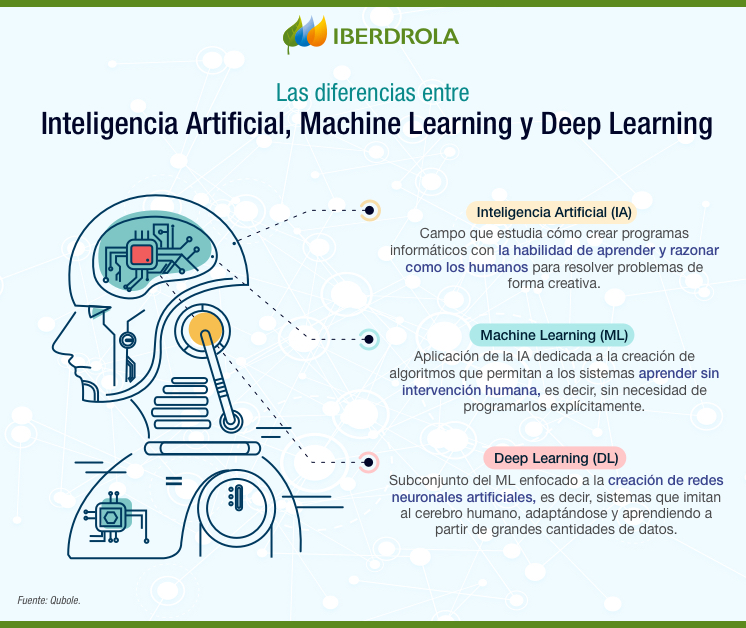
\includegraphics[scale = 1 ]{Deep_Learning_ESP.png}
\caption{\href{https://www.iberdrola.com/innovacion/deep-learning}{iberdrola}}
%\label{}
\end{figure}
\end{frame}

\begin{frame}{Obstáculo}
    Una de las características de nuestra alternativa es que el aprendizaje "Q-learning" sus tiempos tienden a un número muy grande de iteraciones el cual está en contraste con un método metahuerístico.

    \begin{block}<1->{}
        Por último mencionar que nos centraremos  solo en el problema  Flexible Scheduling problem.
    \end{block}
\end{frame}

\begin{frame}{Estado del arte}
Uno de los artículos más importantes es Deep Q-learning for same-day delivery with vehicles and drones \cite{CHEN2022939} presentado por la universidad de Iowa, en el cual se presenta el uso de un DQL (\textit{Deep Q-Learning}) en la búsqueda de rutas óptimas para drones, en dicho artículo no se nos presenta un contraste entre métodos metahuerísticos y el mismo utilizado en dicho artículo, por lo cual si nos sirve de referencia por el uso de Q-Learning, en la búsqueda de rutas, sin embargo esta alejado de lo que presentaremos.
\end{frame}

\begin{frame}{Estado del arte}
	En el artículo Learning to select cuts for efficient mixed-integer programming \cite{HUANG2022108353} se presenta un problema de cortes por medio de Depp-learning, el cual es interesante por el hecho de que vincula problemas de optimización con el uso de aprendizaje deep-learning.
\end{frame}

\begin{frame}{Metodología}
    El diseño estará conformado de inicio, en la implementación de una búsqueda basada en Q-learning, se buscará conectar los resultados en una tabla a  una red neuronal y que por medio de esta misma se de el aprendizaje, después todo esto se aplicará a un problema de flexible job shop scheduling problem.
\end{frame}

\begin{frame}{Metodología}{(Continuación)}
    Lo primero que estamos planeando explorar es el uso de Q-learning, el cual solo hemos podido importar algunas librerías para el uso en problemas de 2-D, los cuales no son muy importantes para lo que tenemos planeado, sin embargo seguimos en la etapa de exploración. \newline

    Lo segundo que queremos es crear una pequeña red neuronal a la que también aplicaremos unas pequeñas pruebas en un problema.
\end{frame}

\begin{frame}{Metodología}{(Continuación)}
    Si logramos esto lo siguiente será introducir unas instancias del problema clásico flexible job shop scheduling problem, en el cual existen ya demasiados resultados con el objetivo  de ver que tan precisos serian nuestros resultados.
\end{frame}

\begin{frame}{Resultados}
Actualmente no se tienen resultados aún, esperamos poder obtenerlos en los próximos tres meses.
\end{frame}

\begin{frame}{Discusión}
La principal pregunta a discusión será: \\ ¿Los resultados obtenidos mejoran algún resultado obtenido por métodos metahuerísticos?
\newline
Sin embargo, antes ya se había mencionado el tiempo es uno de los obstáculos más grande que tenemos, y siguiendo con esta idea tenemos una pregunta más: \\ ¿En qué situaciones podemos encajar el aprendizaje continuo?
\end{frame}

\begin{frame}[allowframebreaks] %allow to expand references to multiple frames (slides)
	\frametitle{References}
	
	\scriptsize{\bibliographystyle{plain}}
	\bibliography{bibliotarea1} %bibtex file name without .bib extension
	
\end{frame}


\end{document}
